% !TEX root = main.tex

One of the main purposes for this project is to explore whether the keywords for spam and ham email changed by year. In this section, we counted the appear frequency of each word as a vector by year respectively. Sort the frequency and find out the top 10 frequent words per year. We would like to explore that whether the frequent words changed by year. Moreover, in the next section, we will use word cloud to visualize the results we found out.\\

According to the Figure.\ref{topwordspam}, although keywords did not change year by year, we still have found out that there might have a difference in 2002. Before 2001, some keywords appreared repeatedly, such as "microsoft", "adobe", "windows", and "free". It seems before 2001, in our data set, the spam emails mostly are related to computer and Microsoft topics. From 2002, "stock", "business", "money", and  "com" become top frequent keywords. We categorize those as economy and Internet topics. \\

For the ham email (Figure. \ref{topwordham}), there is not specific topic for each year. We cannot conclude any specific topic or gap for year. However, overall keywords mainly focus on acadmic, such as "edu", "university", "data". We inferred that ham email data may mostly come from academic organizations.\\

\begin{figure}[H]
    \centering
    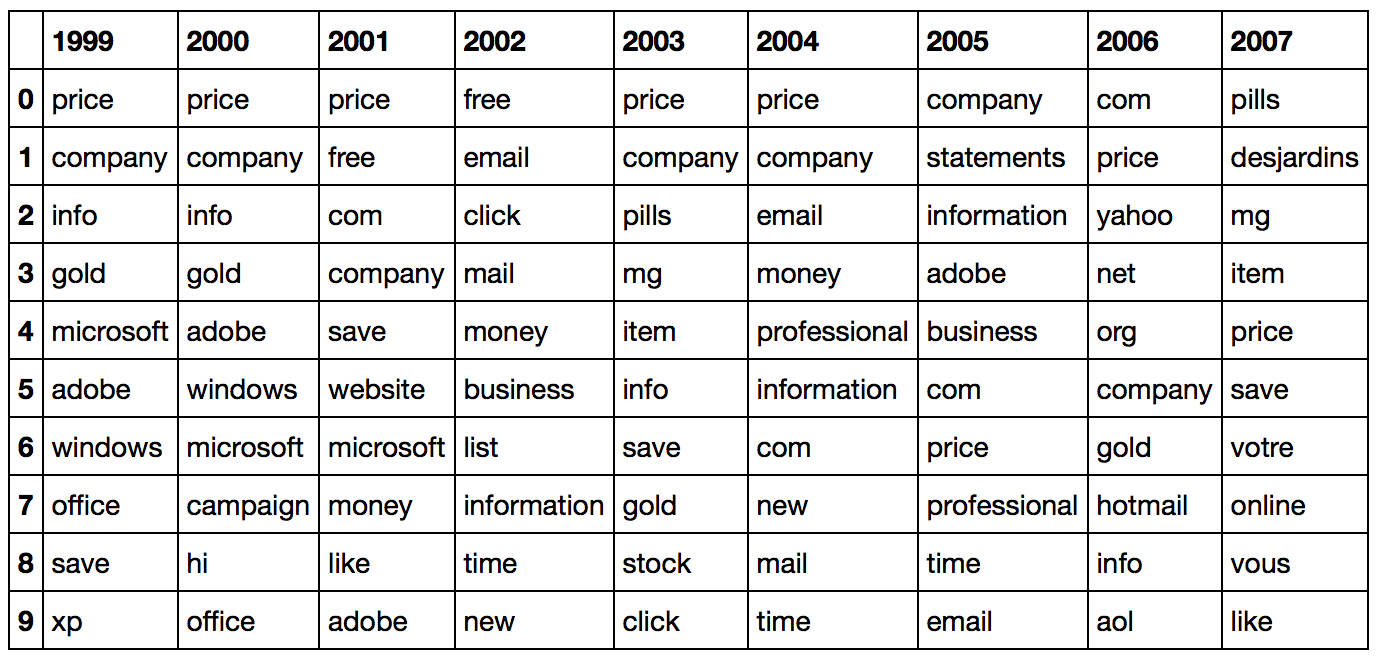
\includegraphics[width=13cm]{top_word_spam.png}
    \caption{Top 10 Frequent Words Of Spam Email}
    \label{topwordspam}
\end{figure}


\begin{figure}[H]
    \centering
    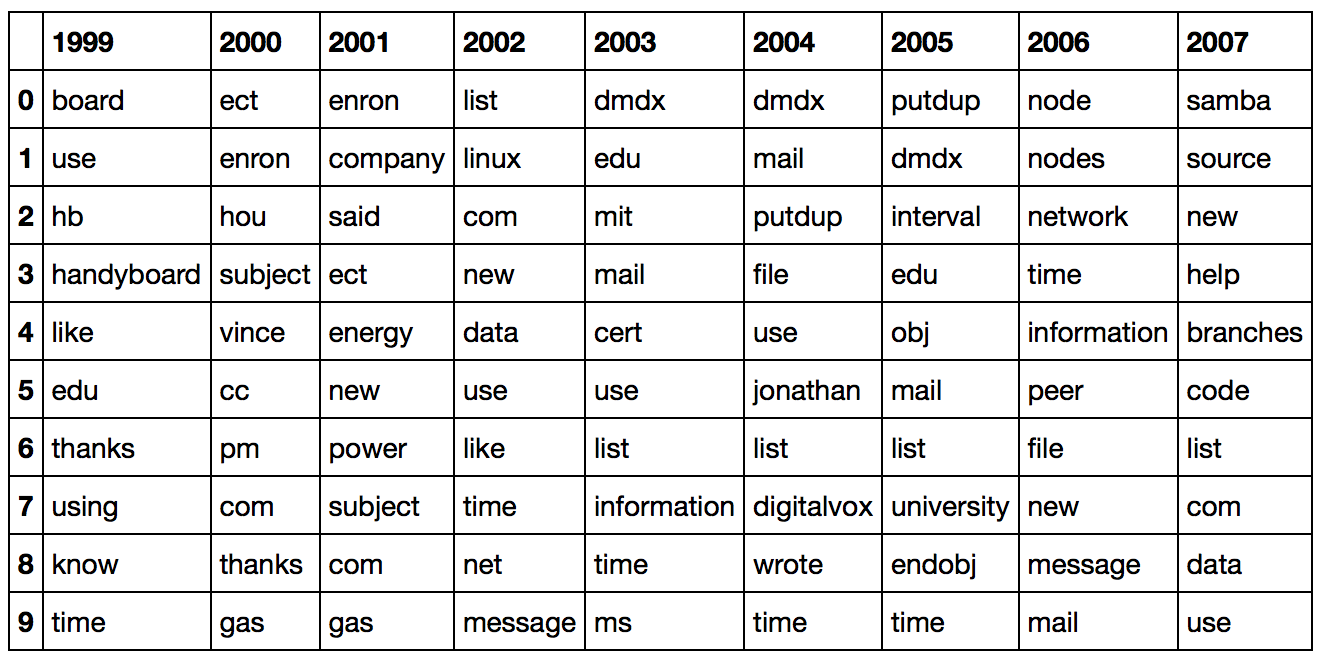
\includegraphics[width=13cm]{top_word_ham.png}
    \caption{Top 10 Frequent Words Of Ham Email}
    \label{topwordham}
\end{figure}


